\section{Conclusion}

\begin{frame}{Open access and education}
    \vspace{-4em}
    \begin{itemize}
        \item Open access: a dedicated portal planned
        \item Education: \textcolor{blue}{\texttt{astroparticle.online}}
    \end{itemize}
    \centering
    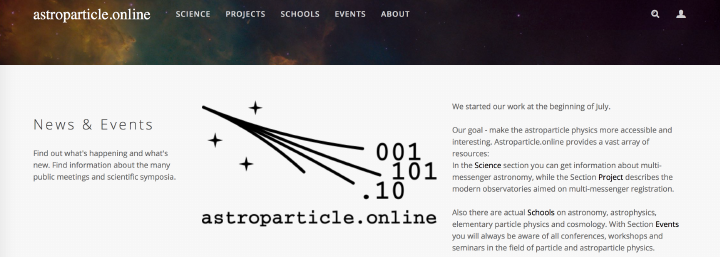
\includegraphics[width=0.85\textwidth]{pics/astro_onl.png}
\end{frame}

\begin{frame}{Outlook}
\textcolor{red}{Translate the bullets (in comments) to English!!!}
    \begin{itemize}
    \item mdl
    \item kcdc
%     \item Нужны инструменты совместного доступа к данным различных экспериментов и эффективный бережный менеджмент этих больших объемов данных
%     \item Консоциум gradlc предлагает концепцию дата инжиниринга в области астропартикл физикс, основанный на уже kcdc. 
%     \item В данный момент производятся работы по созданию aggregation data server'a и совместному анализу данных из экспериментов kascade и taiga;
% \item Доступ к ресурса проекта на данный момент частично предоставлен через портал astroparticle.online.
    \end{itemize}
\end{frame}

% \subsection{The end}
% \begin{frame}{}
%     \begin{center}
%         \textcolor{kit-green100}{\Huge Thank you\\for your attention!\vspace{1em}}  
%         \Large Any questions?
%     \end{center}
% \end{frame}
